%!TEX root = ../main.tex
\section{Introduction} % (fold)
\label{sec:system_analysis}
A thorough system analysis is needed in order to design a system that meets the needs expressed by the use cases. 
This section will present the analysis of the complete system, touching on the following topics:

\begin{itemize}
	\item  \textbf{Parameters of interest:} In order to create a well-suited system it is necessary to gain knowledge of the type of parameters that may be of interest to monitor.
	\item \textbf{Hardware for monitoring parameters:} Having a list of parameters, what hardware is necessary to collect and monitor these parameters.
	\item \textbf{Data rate:} An investigation of the amount of data that can be expected from data producers connected to the system is required.
	\item \textbf{Data collection:} A number of sensors and other data producers is expected to exist on the go-kart.
	It is necessary to analyse how data from these is collected most effectively.
	\item \textbf{Embedded platform:} An investigation of what requirements the platform running the go-kart part of the system should satisfy.
	\item \textbf{Wireless network:} Data is required to be transmitted wirelessly from the go-kart to the monitoring station.
	An investigation of the appropriate technology will be conducted.
	\item \textbf{Local storage:} In order to log data, some form of local storage is required.
	This investigation will examine what options exist on the available platform to choose the appropriate solution.
	\item \textbf{Monitoring station interface:} An analysis of the appropriate interface on the stationary part of the system will be conducted.
\end{itemize}

%!TEX root = ../main.tex

\subsection{Parameters of Interest}
\label{sec:parameters}
In developing new hardware or evaluating current hardware, it is necessary to be able to monitor associated parameters.
This section will investigate what parameters need to be logged in order to provide a useful and complete logging of the behavior of the go-kart.
The parameters in question fall into three categories; Translational parameters, electrical parameters and mechanical parameters.
Clearly, developers may, in addition to the aforementioned categories, also have programmatical information, such as debug information from a motor controller.
This section will deal only with the physical parameters.
The three categories are dealt with in turn in the remainder of this section.
\paragraph*{Physical Parameters}
This category comprises all information about the motion of the go-kart.
\begin{itemize}
	\item \textbf{Position, Absolute:} Providing a means to record the absolute position of the go-kart is a useful feature in certain fields.
	Especially any form of localisation and path finding will be able to put this information to use.
	The absolute position of the go-kart can be recorded using a GPS module or possibly by using a known starting coordinate and information about the relative movement of the go-kart.
	\item \textbf{Position, Relative:} The relative position of the kart can be, as just mentioned, used to infer the absolute position of the go-kart.
	Additionally it can provide a means to analyze a drivers performance on track the or detect drift while cornoring.
	The relative position includes both translational, as well as rotational information.
	This information can be gathered using an inertial measurement unit (IMU).
	An IMU is a compound device, comprised of an accelerometer, a gyroscope and, in some cases, a magnetometer.
	\item \textbf{Velocity:} The velocity of the go-kart is key in optimising lap-times, clearly, it is desirable to monitor this parameter.
	It can be extracted by reading the motor encoders.
	However, the driving wheels are prone to slippage when cornoring, this would give an inaccurate reading of the actual velocity of the go-kart.
	Instead, a simple encoder can be mounted on either one, or both of the front wheels as these are freerunning and independent.
	Once the rotational speed of the axle is known, the velocity of the go-kart can be infered using the tyre diameter.
	\item \textbf{Acceleration:} It may be of interest to monitor the forces exerted on the go-kart, or, its acceleration, as it drives on the track.
	This information is already provided by the accelerometer in the IMU mentioned above and as such provides no additional complication.
\end{itemize}
Three sensors are mentioned in this section.
A GPS, an IMU and an encoder.
In order to limit the scope of the project only the GPS and the IMU will be implemented.
\paragraph*{Electrical Parameters}
This category comprises all information about the electrical aspects of the go-kart.
\begin{itemize}
	\item \textbf{Motor Currents:} Providing a means of monitoring the currents flowing through the motor allows the user to calculate the torque exerted by the motor as well as the current power draw of the motor.
	Knowing the currents could also prove an invaluable debugging tool when developing a new inverter for the go-kart.
	\item \textbf{Throttle Position:} The throttle on the go-kart is connected to a potentiometer.
	Measuring the voltage output of this potentiometer provides a simple way of monitoring the position of the throttle.
	\item \textbf{Desired Currents:} Based on the current throttle position a set of desired currents are calculated.
	Monitoring these allows spotting any discrepancies between the desired and the actual currents.
	\item \textbf{Duty Cycles:} Duty cycle is proportional to the voltage applied to the motor, and can be used to calculate the power going into the motor.
	\item \textbf{Battery Voltage:} As the go-kart is electrical, naturally, it has a battery.
	Monitoring the current battery status could give the user an indication of how much driving time is left, or how long until the batteries are recharged afterwards.
	\item \textbf{Motor Angle:} Knowing the angle of the motor at all times gives a means of more accurately calculate the currents at specific times.
	Additionally, it can be used in Clarke-Parke transformations, again, providing information in debugging an inverter in development.
\end{itemize}
These parameters are all available from the sevcon gen4 motor controller mounted on the go-kart.
This controller has a CANopen interface from which this data can be extracted.
Any users who wish to add their own inverter will simply need to obey the API stated by the sevcon gen4 CANopen interface in order to correctly log the data.
\paragraph*{Mechanical Information}
This category comprises all information about the mechanical aspects of the go-kart.
\begin{itemize}
	\item \textbf{Steering Wheel Angle:} Monitoring the angle of the steering wheel allows analysing the performance of the driver.
	In addition it opens up for the possibility of mechanical control of the go-kart.
	Similarly to monitoring the velocity, the steering wheel angle can be monitored by adding an encoder to the steering column.
	\item \textbf{Braking Pedal Position:} The braking system on the go-kart is similar to that of an ordinary car.
	The braking disc is mounted on the driving axle and the braking calibers connected to the brake pedal by a series of oil-filled hoses.
	Monitoring its actuation allows analysing the performance of the driver and as mentioned above, may potentially allow for mechanical control of the go-kart
	\item \textbf{Temperature:} Certain parts of the go-kart directly impact driving performance with changing temperature.
	Additionally, overheating the motor, the batteries or other components may cause expensive or dangerous failures.
\end{itemize}
As both monitoring of the steering wheel angle and the braking pedal position would require mechanical changes to the go-kart, they are beyond the scope of this project and as such will not be implemented.

\subsubsection*{Conclusion}
As mentioned in the beginning of the section, the parameters discussed throughout this section are limited to those that explain the physical aspects of the go-kart.
A future project may wish to introduce a data producer which does not directly gather data from a sensor, but generates a filtered output of other sensory equipment.
It is not possible to account for every parameter that a future developer may wish to add.
In order to provide a proof of concept for the system it was decided to implement the control for three data producers; the Sevcon Gen4 motor controller, an IMU and a GPS.

\subsection{Hardware for Monitoring Parameters}
\label{sec:hardware_for_par}
In section \ref{sec:parameters} an overview of the different parameters that may be of interest for logging is given.
It was concluded that three components would suffice as a proof of concept; the Sevcon Gen4 motor controller, an IMU and a GPS.
This section will explore in more detail what requirements and communication schemes that exist for each of the components.

\subsubsection*{Sevcon Gen4 Motor Controller}
\label{sec:interfacin_with_sevcon}

The Sevcon Gen4 motor driver is a general purpose AC motor driver. 
This means, it can be used for both asynchronous and synchronous motors of a wide range of sizes.
The controller can then be set up for the particular motor and peripherals, and run without interfacing to another computer.
However, it is also possible to read data from it while running, and in some cases set values.
It is therefore possible to use this to access the electrical parameters. \\

The Sevcon communicates through CANopen, which is a high level protocol running on top of CAN.
This allows reading from and writing to a vast array of registers of varying length, which is described in further detail on page pageref~\ref{sub:CANopen}\\

\subsubsection*{Inertial Measurement Unit (IMU)}
\label{sec:imu}
\mikkel{Maybe remove all requirements because we just took the availabl sensors}
IMU's, generally, exist in two versions.
A 6D and a 9D version (Dimensions).
Both include an accelerometer and a gyroscope, each adding three dimensions.
In addition to these the 9D IMU includes a magnetometer, enabling measurement of absolute direction, as opposed to the relative measurement of direction given by the gyroscope.
The requirement in terms of each of these parts is given as:
\begin{itemize}
	\item \textbf{Accelerometer [\si{\metre\per\second^2}]:} As the name implies, the accelerometer measures accelerations.
	That is, when the component changes velocity the acceleration exerted on the IMU is measured.
	Professional drivers using professional grade go karts driving upwards of 250 \si{\kilo\metre\per\hour} can reach up to 2-3 g's of force exerted on them.
	The go kart available in this project has a maximum speed of 50 \si{\kilo\metre\per\hour}.
	Clearly, the forces exerted on this platform will be lower, however, a minimum requirement of $\pm$ 3g will be set for the accelerometer in the IMU.
	This will ensure that bumps in the road doesn't saturate the accelerometer
	\item \textbf{Gyroscope [\si{\degree\per\second}]:} 
	A gyroscope in this sense consists of three gyroscopes spinning at high velocity.
	When the IMU turns in around any of its axis, the change will be detected on one of the gyroscopes. 
	The gyroscope part of the IMU will mostly be useful for detecting change in inclination, turning the go kart, or spinning out.
	In the two former cases, the rate of change is fairly low, about 90 \si{\degree\per\second} for a sharp turn. 
	But in case the driver spins out, or oversteers, this number is much higher. 
	Therefore the minimum requirement of $\pm 360 \si{\degree\per\second}$.
	\item \textbf{Magnetometer [\si{\tesla}]:} 
	The magnetometer measures the magnetic flux density through the IMU.
	This is done by three hall sensors measuring the flux density along three axis. 
	This can be used to calculate the absolute orientation of the go-kart, both which way is north and which way is up.
	This type of sensor is notoriously noise sensitive.
	The flux density of the Earth's magnetic field ranges up to $65 \si{\micro\tesla}$.
	By comparison, this is several orders of magnitude lower than the magnetic field generated by the motor, so it's important to place the IMU away from the motor and high power wires.
	The scale of the magnetometer would need to be at least $\pm 75 \si{\micro \tesla}$.
\end{itemize}
Common for all sensors is, that the smallest range, that is larger than the requirements above, is preferred, as these will have finer resolution, while keeping the bitrate down.
The accelerometer measures the second derivative of translation with respect to time. 
The gyroscope measures the first derivative of rotation with respect to time.
This leaves three elements, that can be calculated: absolute translation (position), first derivative of translation (speed), absolute rotation (yaw, pitch and roll) and second derivative of rotation.
The absolute translation is measured by the GPS, and the others can be calculated by data fusion of the IMU measurements.\\

VN-100 from Vectornav is a 9D IMU with built in data processing to deduce more elements, that are not directly measurable.
Its ranges are generally much larger than the requirements, but at the same time, has fine enough resolution.
The accelerometer: 16 bits,  $\pm 16 \si{\meter \per \second \squared}$

\begin{table}
	\centering
	\begin{tabular}{ c | c c c}
		{\textbf{Sensor}} & {\textbf{Range}} & {\textbf{Bit}} & {\textbf{LSB}}\\
		\hline
		{Accelerometer}	& { $\pm 16 \mathrm{g}$}					& {16}	& {$< 0.5 \mathrm{g}$}\\
		{Gyroscope}		& { $\pm 2000\si{\degree \per \second}$ }	& {18}	& {$<0.02 \si{\degree \per \second}$}\\
		{Magnetometer}	& { $\pm 250 \si{\micro \tesla}$}			& {12}	& {$0.15 \si{\micro \tesla}$}
	\end{tabular}
	\caption{List of the resolution of the internal ADCs on the Vectornav VN-100}
	\label{tab:vectornav_measurement_resolution}
\end{table}

In addition to the IMU sensors, the VN-100 also records air pressure, which is of no concern to us.
Apart from the raw data listed above, the VN-100 can calculate other parameters, such as quaternions, yaw, pitch, roll, absolute heading and altitude.
I can also make the accelerometer data zero base, meaning when the go kart is standing still, 0g will be printed from the IMU, rather than the 1g caused by the gravitational pull of earth. \\

The Vectornav comes in a rugged, waterproof casing with a USB cable going out.
Drivers are available on Linux, where one can easily call functions to return the latest values on multiple axes at the same time.

\subsubsection*{Global Positioning System (GPS)}
\mikkel{Something here?}
A GPS sensor is included on the Go Kart. 
The purpose of this is to give absolute position readings at fixed intervals, much like a runner would be able to see their route on a map afterwards.
However unlike a runner, a go kart is not supposed to drive at a constant speed nor in a straight line, and as such a GPS is likely too slow to be used on it's own.
The update rate of the position depends on the rate of messages sent out which is several seconds, which means that the GPS location is update at best a few times per second. 
The only parameter is then really the precision. \\

It was possible to borrow a GPS sensor from U-blox from Kjeld Jensen, the NEO-6P.
This has a data rate of 5 Hz, and a Circular Error Probability (CEP) of down to 2 m.
This means, that any position measurement has a 50 \% chance of being within a radius of 2 m from the actual position. 
This is very good compared to other GPS modules, but is barely precise enough to determine which side of a go kart track, the Go Kart starts in. 
Further precision is however a possibility using a base station, solutions, that U-blox does offer.\\

This is a tremendously good GPS module, and will give a good platform for data fusion, should later semester project want to work with this. 
One downside however is, that it only uses GPS, and not GLONASS or Galileo, which inherently limits the number of satellites visible to the node at any one point. 
Furthermore, a GPS module would only work outdoors, and the nearest Go Kart course to here is indoor, in which case a local position system would be preferred.\\

The U-blox NEO-6P is mounted on a custom made PCB with a min USB port and a connector for the antenna. 
Drivers are available for Linux, so that a stream of messages can be read out and converted to the correct data format.
\martin{verification}

\subsubsection*{Conclusion}
\todo[inline]{Table with chosen sensors and their interfaces}

\begin{table}[H]
	\centering
	\begin{tabular}{|l|l|l|}
		\hline
		\textbf{Sensor} & \textbf{Brand} & \textbf{Interface} \\
		\hline
		Motor controller & Sevcon Gen4 & CAN open \\ 
		\hline
		IMU & Vectornav VN-100 & USB, drivers for Linux\\
		\hline
		GPS & U-blox NEO-6p & USB, drivers for Linux\\
		\hline
		
	\end{tabular}
\end{table}


%!TEX root = ../main.tex

\subsection{Data Rate}
Which architecture is most suitable for the system is largely dependent on the amount of data that it has to support.
This section will explore the amount of data that can be expected from a data producer connected to the system.
\\~\\
Many of these parameters pose different requirements in terms of the desired sample rate as well as the size of each sample.
A temperature sensor, for instance, does not require nearly the same sampling frequency as an accelerometer.
Due to these differences the data rate expected from one data producer may differ wildly from another.
In order to provide a safe estimate, the expected data rate is calculated using a "worst-case" sensor.
That is, the type of sensor which set the highest requirements in terms of sampling frequency as well as data size.
Again, it is not possible to foresee every application that may be developed in the future.
Despite of this the IMU chosen for this project, see section~\ref{sec:imu}, is considered as the worst-case.
It is is a 10-axis sensor that provides data at a rate up to 300\si{\hertz} at 32 bit floating point precision.
This would result in a data rate of:

$$300\cdot32\cdot10=96\,\text{Kb/s}$$

As previously mentioned, this is the assumed worst case for the system.
As such there may be only a few data producers providing data at this rate.
Most other producers will provide only limited data in relation to the IMU, either due to a much lower sampling frequency or an overall smaller data size.
A GPS generally provides an update only at a few \si{\hertz}. 
An encoder, while it may have a reasonably high sampling rate, it is most likely not close to 32 bit resolution.
\\~\\
Assuming five sensors running at the assumed worst-case rate and ten running at half that rate, the resulting data rate will be 960 Kb/s or approximately 1 Mb/s.

% \subsection{Data Logging}
% \todo[inline]{Mikkel: Should maybe change name?}
% A feature will be data logging. 
% Any data could be put into the log, although some signals can be logged at significantly higher rates than others
% If all data is recorded at the fastest rate, this could present a storage problem.
% This challenge will be analyzed here.

% \subsubsection{Sample Rate}
% Datalogging should be useful for working with an inverter as was the case on the first semester.
% Likely it would be interesting to log the phase-current to the motor at high enough rate to accurately depict their sinusoidal short term average.
% The ripple current or voltage at the motor terminals should be measured in the lab, as this requires a high sample rate, and more control than offered on the test track.
% This data logging would be useful for recording current in the motor as the go kart is driving.
% Additionally it would be relevant to record the encoder output, and possibly the DC voltage at the input of the inverter and the duty for each phase.
% Only the currents are bound to change rapidly, and as such they determine the minimum acceptable sample rate.
% By looking at the maximum frequency of the motor and the most extreme rate of change permissible by the armature inductance, it is possible to set a sample rate for the log file.\\

% According to the manufacturer of the motor, the maximum rotational velocity is 5000 RPM.
% With four pole pairs, this comes to a maximum sinusoidal frequency of 333 Hz. 
% It is not necessary to record at a rate significantly larger than the Nyquist limit in order to adequately record the sinusoidal.
% Simulations show, that by using Clark-Park transformation, interpolation and then the inverse Clarke-Park transformation, there is nearly no difference between a low sample rate of $1\si{\kilo\hertz}$, and a higher sample rate of $3.3\si{\kilo\hertz}$, as shown below.

% \begin{figure}
% 	\centering
% 	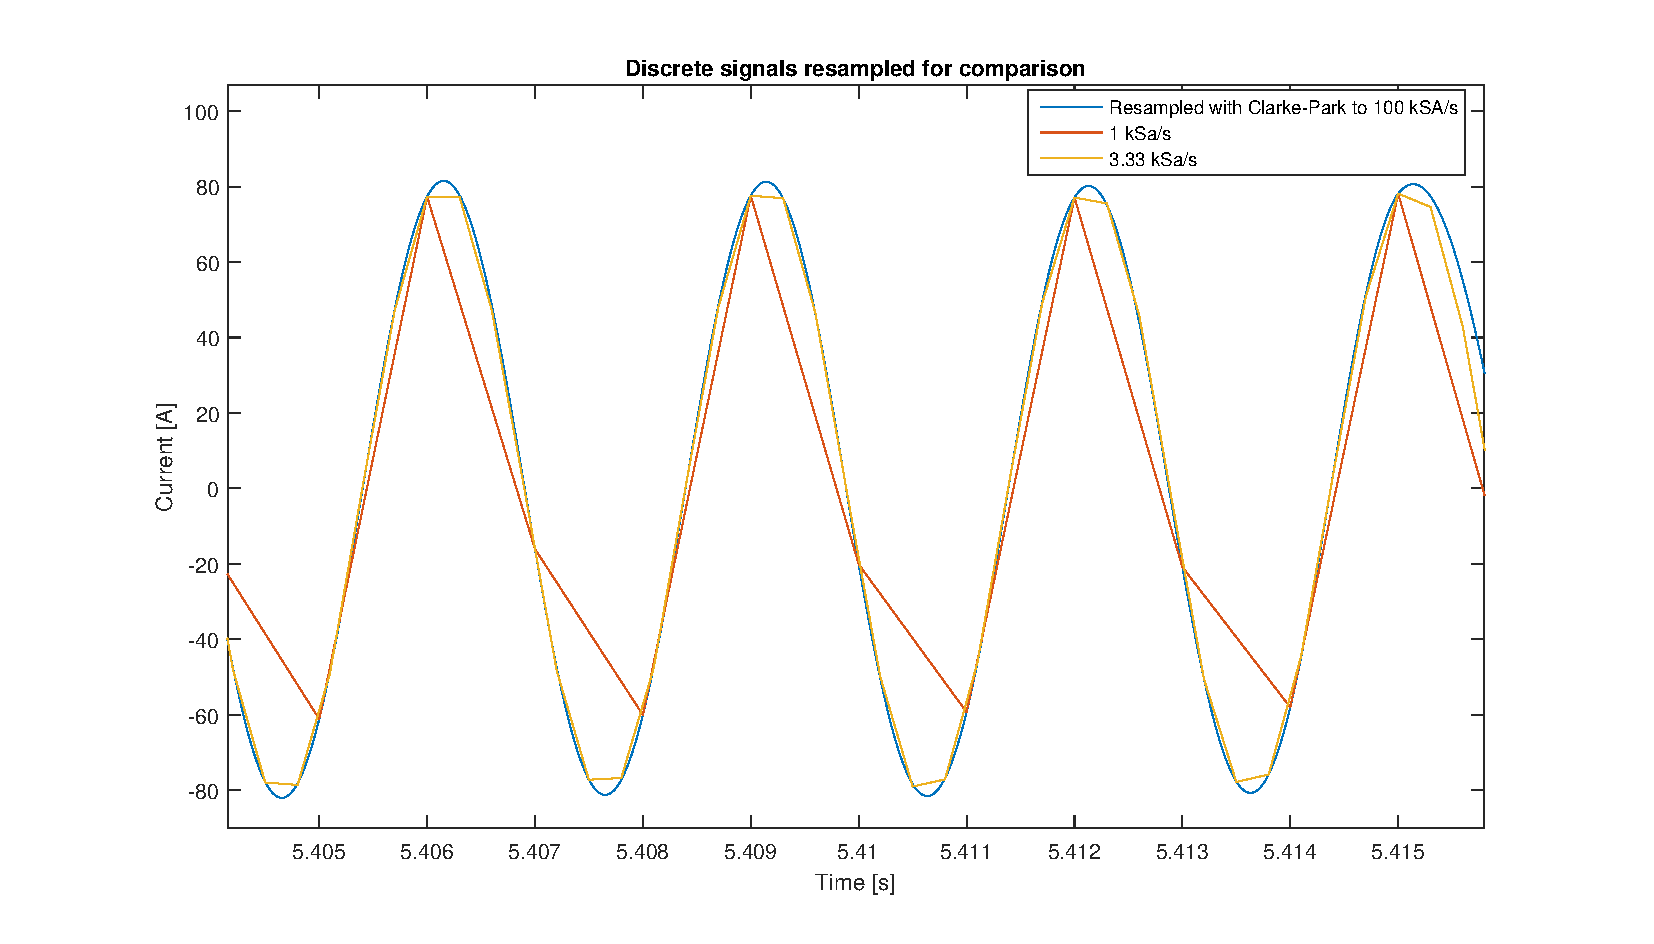
\includegraphics[width = 0.9\linewidth]{graphics/Clarke-park_resampled}	
% 	\caption{Comparison of data recorded at 1 kSa/s and 3.33 kSa/s, against 100 kSa/s resampled using Clarke-Park}
% 	\label{fig:Clarke-park_resampled}
% \end{figure}

% The resampled data from the 1 kSa/s and 3.3 kSa/s (orange and purple respectively on figure\ref{fig:Clarke-park_resampled}) are almost identical.
% However, there is a small visible difference around the time 5.527 s, likely due to the limited precision of the encoder.
% This also doesn't take into account any disturbance or noise, which could make it hard to reconstruct the signals with lower sample rates.\\

% Additionally, the Matlab function, resample, produces nicely filtered vectors with smaller time steps, so it is possible to use a low sample rate for time invariant signals.\\
% Another way to look at this is to calculate the maximum change in current from one sample to another.
% This is determined by the inductance of the motor, which is $600 \si{\micro \henry}$ \todo[inline]{when one half bridge is high, and the two others are low, it's one armature inductance of 400 uH in series with two parallel armature inductances}, and the maximum voltage across it, which is $V_{BAT}=52.8 \si{\volt}$. 
% At a sample rate of 3.33 kSa/s, this results in a theoretical maximum step of $264\si{\ampere}$.
% A sample rate lower than this, would make it hard to properly record such sudden steps.

% \subsubsection{Data Type}
% When the sample rate is known, it is possible to get an estimate of how much storage space would be needed. 
% It would be easiest, and most useful, to record using simple comma separated files, but these tend to take up more space than necessary.
% The analog input to the Zybo are 12 bit, which means, that full precision of these would be possible with 4 digits, and often a decimal point and potentially a negative sign.
% Including the horizontal separator, this comes to 6.5 bytes per point.\\

% An example of recording could include time, two currents, a voltage and the encoder output, as displayed below
% \begin{lstlisting}
% Time	Ia	Ib	V	Encoder
% 1.0000	052.3	-278.1	52.56	16
% 1.0003	057.7	-280.4	52.54	17
% \end{lstlisting}
% That brings each line length to 32 bytes (8 bytes for time, 5.5 for the three analog, 3 bytes for encoder, 5 for separators).
% At a sample rate of 3.33 kSa/s, this comes to 6.1MB per minute. 
% With the current SD cards having 4 GB of free un-partitioned space, this gives up to 11 hours of recording time.\\

% Alternately, it is possible to invent a file structure, that allows several arrays of with different data types.
% By storing numbers in binary files instead of text, it is possible to reduce the space requirements to a third (2 bytes per analog, 4 bytes per timestamp (allowing up to 49 days of ms), and 1 byte for encoder).
% This however will reduce the readability greatly, and include the workload, as one will need to write code both for encoding and decoding the file. \\

% Since this is out of the scope of this project, and the sample rate isn't larger than it is, logging in standard ASCII will suffice.
% Likely, different sample rates will be recorded to different log files

%!TEX root = ../main.tex

\section{Data Collection}
\label{sec:data_collection}
As described in previous sections, the system will have to support the use of several data producers.
In addition to this, it should also be possible to easily add additional data producers at a later time.
It is possible to implement the support of many producers on a single platform, however, eventually the platform would likely run out of I/O for additional support.
The single-platform approach would also likely not meet the computational requirements set by the increasing amount of equipment.
This implies that a multi-platform system is the appropriate approach for this system.
Each platform, or node, would then implement the functionality of one or more data producers.\\

The data needs to be collected from all of the nodes, then logged and transmitted wirelessly to the monitoring station.
The type of network depends greatly on the number of nodes that it has to support.
An ongoing project on SDU, Formula Student \cite{formulastudent}, has a similar platform for which a network has been developed.
That project, which is to develop a race car, has a network of seven physical nodes, distributed around the car, which each handle data producers and consumers in that area.
The physical distribution of the nodes means that the responsibility of a given group of sensors can be given to a node based on their placement on the car.
The parameters found in section \ref{sec:parameters} can be measured using five different types of sensors.
This project does, however, aim to give users the ability to add their own nodes.
For this reason the limit of supported nodes is set to 16.
It is worth noting that the structure of each node is irrelevant, so long as it adheres to the networks communication standards.
This means that a node can potentially comprise several (different) sensors or perhaps a complete separate network of nodes.

\subsection{Network Topology}

There are various network topologies that can be used to setup the required node network for this project.
These include among others the bus, ring and star. 
Before choosing a topology, a brief description of the purpose and functionality of the network as well as an overview of their advantages and disadvantages are needed.\\ 

The purpose of this network is to accommodate multiple nodes, such as sensors, sub-networks and in general data-producers.
These nodes need to be able to transfer their data and receive commands, as specified in the use cases.
\\
The communication between the various nodes does not require a central hub.
Furthermore, in the case that one node fails, the network as a whole should still be operative.
Since it is a multi-node network and it may require more nodes in the future, scalability is also required.

\subsubsection*{Network Topologies}
Networks can be described by different patterns, or topologies, some of which might have several technologies.
Some of these topologies, that are practical to implement, are listed bellow.
\begin{itemize}
\item \textbf{Bus:}
On this network, all nodes communicate through a common bus. 
This means that one node communicates to all other nodes at the same time, and that only one node can transmit at a time.
\item \textbf{Ring:} All the nodes in this type of network form a ring, where each node is connected to its two neighbours.
Messages travel along the ring.
\item \textbf{Star:} The star topology is a centralized type of networking.
All nodes are connected to a central hub, handling all the communication between them.
It offers high bandwidth and is easy to implement.
The major disadvantage is that if the hub fails, the entire network fails.
It can be scalable to a certain point, since the hub can be upgraded to handle more connections.
\end{itemize}

\subsubsection*{Suitable Topology}
%\martin{Like i todo'ed above, we should only concern ourselves with bus, ring and star, and at this point we should come to the conclusion that star does not work, and that ring and bus is really a toss up.}
\martin{rewrite}
For the system's networking purpose, the mesh type is not suitable, since it adds extra hardware requirements.
A node may be a simple sensor with a small micro controller and hence, connecting it to such a network is not feasible.
%In our system, a small embedded board computer will be the ov-computer which requires to maintain its connection with the network even in case of failures and also possibly the central hub in centralized topologies that such as the star and the tree.
The star network requires a lot of connections which normally are not present at standard micro controllers.
%Thus, these two topologies are not suited, since in case of its failure, the whole network fails.
Thus, the mesh and star networks are not suited for this system.
Scalability is also a requirement for the future connection of nodes.
Although the majority of the types provide a level of scalability, the addition of extra nodes always decrease the overall performance of any network.
Hence, a topology that balances the decrease in performance against the network's expansion is best suited for the project.\\
\martin{bus and ring fits best, subnetworks are irrelevant}
The approach that fits the requirements is implementing a bus network, where each node may be a subnetwork of a different type depending on the needs, making it into a hybrid network having a bus topology as its basis.
This type provides a good balance of reliability, scalability, hardware requirements and communication speed in comparison to the others.
\subsection{Networking technology}
In the previous section it was found that the bus and ring topologies in particular lend themselves well to the implementation of this system.
A number of different technologies exist, that implement these topologies. 
This section explores a few of the ones that are considered for this project to find the one best suited.

\subsubsection*{Selecting Technologies}
Different networking technologies exist in use today, such as CAN and Powerlink among others.
Powerlink is the network topology used by Formula Student; it is a ring type network, using Ethernet between neighbouring nodes.
Messages are transmitted as a pulse train from one node to its neighbour, who then appends its data to the end of this train. 
Message trains are sent out at fixed time intervals.
However, message trains need to be fully received by one node before it can be transmitted with its data appended, and because of this it can be an issue synchronizing the nodes.
There can be very little overhead, and with the Ethernet cables and ports setting the limits, the bandwidth is very large -- 100 MB/s on Formula Student.
However, this does require all nodes to have two Ethernet ports with direct access to an FPGA, and that is rare to find on an evaluation board.\\

CAN is a bus topology widely used in the automotive industry with data rates up to 1Mbit/s for small network lengths.
This is slightly less than the requirement calculated in section~\ref{sec:data_rate}, however that number was based on the highest possible sample rate of the IMU, along with the inefficient data type, which is 32 bit float.
Because CAN is a bus topology, it is easy to add another node to the bus, as one would just tap into the bus anywhere.
It is because of this tapping into the bus, that it is not suitable for higher data rates, and if the bus breaks at any one point, communication is lost on the entire bus.
Unlike Powerlink, this runs without a dedicated master.
It is not nearly as fast as Powerlink, and does not have the redundancy of a ring network.
Due to the use of buffers, the CAN bus is not a real time bus, but synchronization is easier.\\

The open source project openPowerlink offers FPGA implementation of Powerlink, and external modules can be utilized to handle the hardware part of the network.
This will allow evaluation boards with less than two Ethernet ports to work in the ring network. 
CAN also requires one external piece of hardware, but does not necessarily require an FPGA to run. 
According to the data rate calculations in section~\ref{sec:data_rate}, the CAN network has enough bandwidth to handle the requirements of this project. 
Because it is easier to implement CAN, and to add nodes to it, it has been decided to use a CAN network.
\martin{easer because less hardware, cheaper, powerlink is propriatary}

%!TEX root = ../main.tex

\subsection{Controller Area Network (CAN)}\label{sec:canbusanalysis}
The CAN protocol was originally developed in the 1980's by Bosch.
It is a multi-master network, where each node connects to a common bus.
All nodes are able to broadcast data to all other nodes.
The CAN protocol includes an overhead of 47 bits per message.
The data sent in a message can vary in size from 0 to 8 bytes.
This is described in detail in section~\ref{sub:CanMessageFrame}.
The bus offers 1 Mbit/s at up 40 \si{\metre} of length.

\begin{figure}[h!]
	\centering
	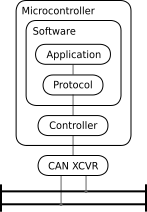
\includegraphics{graphics/canbus_setup}
	\caption{CAN node architecture}
	\label{fig:canbus_setup}
\end{figure}

Some hardware is necessary in order to properly realise a CAN network.
The structure of each node can be seen in figure~\ref{fig:canbus_setup}.
The following paragraphs explain the physical parts of this structure as well as the requirements of the protocol.

\subsubsection*{The CAN Bus}
The bus is shown in figure~\ref{fig:analysisnodes}.
It is a differential voltage bus.
This means that the value on the bus is determined by the voltage difference between the two wires, rather than the absolute voltage of either wire.
The bus has to be made with twisted pair wires with a characteristic impedance of $\si{120 \ohm}$ and terminated at each end with $\si{120 \ohm}$ resistors.
This increases the EMC of the bus, as inductive noise present on one wire is likely also present on the other, and the noise will cancel itself out.\\

Because it iss a differential bus, if the bus is broken at any point, no communication will be received, even if the receiving node still has a galvanic connection to the transmitting node.
Alternatively, it is possible to terminate each node, but this greatly reduces transmission speed.

\begin{figure}[h]
	\centering
	\includegraphics[width=.75\linewidth]{graphics/analysis_nodes}
	\caption{Overview of the network structure.}
	\label{fig:analysisnodes}
\end{figure}

\subsubsection*{The CAN Transceiver (XCVR)}
As CAN uses differential voltages, it is not possible to implement directly in micro controllers.
Typically a micro controller has digital ports putting out either $ 0 \si{\volt}$, or a fixed voltage level defined as high.
That is, depending on the voltage level, the signal is perceived as either high or low.
As mentioned above, the absolute voltage of either wire of the CAN bus does not matter, but difference in voltage does. 
As there are multiple nodes on the same bus, it is also important for one node to be able to dominate the others.
Specifically for CAN, \texttt{0} is dominant, which means if one node tries to transmit \texttt{1} while another node transmits \texttt{0}, the \texttt{0} is transmitted.
By checking if the bus matches what a node transmits, it can detect if there is another dominant node occupying the bus.\\

The transceivers translate the Tx signal from the CAN controller to the differential bus signal, and simultaneously translates the bus signal to the Rx signal going into the controller.
That means, that while a node is sending, Tx and Rx are the same.

\subsubsection*{The CAN Controller}
This element can be standalone hardware, but it is in many cases built into the micro controller.
If the CAN controller notices that the Rx it receives is not the same as the Tx it sends out, it will know that it is being dominated.
Due to the tight timing demands, this cannot be implemented in software.
The major advantage of having the controller built into the micro controller is that it would otherwise require additional communication, like UART or SPI, for the communication between the microprocessor and controller.
A CAN controller (both standalone and built-in) has an input and output FIFO, meaning that the CAN bus communication can operate asynchronously.
This does, however, mean that it can not be used as a real time network.
Asynchronous operation is necessary as there is only one bus and it is possible that nodes will attempt to transmit messages simultaneously.

\subsubsection*{Protocol}
The CAN standard, apart from a variety of hardware requirements, also defines a protocol that nodes on a CAN bus should adhere to.
Part of this protocol is a well defined message frame.
A detailed description of this frame can be seen in section \ref{sub:CanMessageFrame}.\\

It should be possible to toggle the data collection of individual nodes.
This means that it is necessary to have a protocol that allows addressing each node on the bus individually.
The message frame of the CAN protocol does include a message ID, however this ID holds no information about the sender of the message.
In CAN a table of all message ID's and their meaning is used to decode messages.
Achieving the desired functionality will require an adaptation of the protocol. \\

One such adaption already exists in the form of CANopen.
CANopen is a widely used standard that builds upon CAN.
\cite{CANopen_introduction} shows that CAN accounts for the physical and data-link layers in the OSI model while CANopen accounts for the network to application layer.
It is already used in the communication with the Sevcon Gen4 and as such, using this protocol would mean that the Sevcon could be connected directly on the bus.
CANopen is quite extensive, implementing many features that are not necessarily beneficial in this application.
The many features also adds to the complexity of learning how to use the system.
It also adds a significant amount of overhead for each message, taking up bandwidth which could have otherwise been used for data.\\

Another option is to create a custom protocol, using CAN as the physical and data-link layers.
Designing a custom protocol means that the overhead can be reduced to the bare minimum.
This would allow for a smaller, simpler protocol.
As described in section \ref{sec:data_collection}, the protocol should support up to 16 nodes and allow for addition of new nodes.
Since it is required to toggle the data production from a node, it should also be possible to address every node individually.

Due to the added complexity and overhead of CANopen, it is decided to develop a custom protocol. 
This is explored in depth in section~\ref{sub:CAN_protocol}.
In that section, it is also being described why CANopen is a not an ideal fit for this project.
\thomas{described in more detail}
\todo[inline]{I changed this. Martin.}


%!TEX root = ../main.tex

\section{Embedded Platform}\label{sec:EP}
As described in section \ref{sec:data_collection}, a CAN network will be created to support the nodes on the go-kart.
Each node is some type of embedded platform (EP), possibly connected to a sensor or other data producing unit.
From the perspective of the network the only requirement for the EP is that it has a CAN controller.
In principle the network could consist of 16 different EP's.
\subsection{Nodes}
In section \ref{sec:hardware_for_par}, it was chosen to use an IMU and a GPS, both using a USB interface.
Additionally, one node has to transfer data wirelessly from the go-kart to a stationary monitoring system.
It was chosen to use wifi as the wireless protocol, and this will be handled on a separate node.
As the wifi node provides the link to the laptop, it is natural to make this the master node.
\martin{I declared the wifi node as the master. Is this premature? Or too late? FYI, section~\ref{sec:wireless_analysis} determines that it is in fact WiFi}
Both USB and wifi are implemented in most Linux operating systems.
Thus choosing an EP supporting such an operating system will greatly simplify the code that needs to be written for all nodes.
The authors attend a course on software development in Linux, as such, this is a natural choice.
\\
As a part of the aforementioned course, the authors have access to the Zybo.
This platform fits the requirements set for a node and being accessible, this is the EP chosen for the project.

\subsection{Zynq Board (Zybo)}
The Zybo has a Xilinx Zynq Z-7010 chip, which has a processing system (PS) part and a programmable logic (PL) part.
The PS consists of a dual-core ARM Cortex-A9 processor and I/O peripherals, including two CAN controllers and USB.
The PL consists of a Xilinx 7-series Field Programmable Gate Array (FPGA). 
The PL and PS are connected through a bus called AXI.
The Zybo itself is made as a development platform with several buttons, switches, LEDs, connections for USB, Ethernet, HDMI and several PMOD connectors.
\thomas{Look for zybo board, replace with zybo}
\subsubsection{Linux on the Zybo}
Several Linux distribution are configured to run on the Zybo. 
The authors have experience with the Xillinux \footnote{http://xillybus.com/xillinux} distribution, therefore this will be used.
Xillinux is based upon the digilent Linux distribution which is built on the Xilinx distribution which is based upon Ubuntu 12.04.
In the Xillinux architecture there is a DMA-based bus between the PL and PS called Xillybus.
Xillybus is implemented as an IP core in PL and a corresponding Xillybus driver in the Xillinux kernel.
In PL the IP core is interfaced through standard FIFO buffers.
In PS the Xillybus is reached in userspace through \textit{"/dev/xillybus\_<bus-name>"}.
\mikkel{Should there be a figure showing PS and PL on the ZYBO?}

\subsection{Power Requirements}\label{sec:power_requirements}
The Zybos need to be supplied with 5 V, which subsequently powers the sensors, the CAN busses and any other peripherals present on the go-kart.
The Sevcon has a 5V output capable of supplying up to $\si{100 \milli \ampere}$, which is insufficient.
It is therefore necessary to use a DC-DC converter to supply the nodes.
Some tests along with datasheet lookups are used to determine the power requirements for the system.\\

By measurement, it was found that one Zybo draws a maximum of $\si{475 \milli \ampere}$ while running Linux.
The CAN transceivers consume up to 40 mA\cite{3.3V_CAN}. 
The GPS module consumes up to 40 mA, the IMU consumes up to 56 mA. 
Generally it is assumed that the sensors do not consume more than 75 mA per node, which brings the total current consumption up to 600 mA.
For 16 nodes, this brings the total current up to 9.6 A.\\

The source for this DC-DC converter will be the batteries on the go-kart. 
These vary depending on charge from 57.6 down to 40 V, so the DC-DC converter would need to be operable in this entire range.


\begin{table}[H]
	\centering
	\begin{tabular}{r|l}
		Parameter & Requirement  \\
		\hline
		Input voltage & 40-57.6\\
		Output voltage & 5 \\
		Output Current & 9.6
	\end{tabular}
\end{table}


\subsection{Conclusion}
A node is not hardware specific. 
It can be run on any type of embedded platform, so long as it is cabable of communication over CAN.
Throughout this project the nodes will be run on the Zybo platform.
This will ease the development as Linux includes support for both USB and wifi.
It was found that a fully populated system will draw at upwards of 10\si{\ampere}.

%!TEX root = ../main.tex

\section{Wireless transmission}
Communication between the go-kart and the monitoring station is required to happen wirelessly.
This section aims to determine what requirements exist for the wireless connection. 
Upon determining the requirements, a suitable technology will be found.

\subsection{Range}
The range of the transmission is determined by the length of the test track. 
Normally the SDU kart is tested on one of the parking lots at SDU.
This "track" is 50\si{\metre} long and 20\si{\metre} wide.
There are no appreciable obstacles for the transmission on the parking lot. 
This test track sets a minimum requirement that the wireless setup should be able to transmit data at 55m with no obstacles.
\\
Actual go-kart tracks are usually larger than the parking lot in question though. 
The nearest go-kart track is \textit{Odense gokart Hal}, which is also thought to be an average size indoor go-kart track.
The track is about 70m long and 40m in width with no obstacles other than the barriers. 
If the wireless transmitter and receiver are placed above the barriers then the barriers will not be an obstruction to the transmission. 
This track sets a minimum requirement of at least 80m transmission.

\subsection{Bandwidth}
The CANbus has a bandwidth of up to 1Mbit/s.
The wireless technology therefore has to at least match this figure reliably.
%Data is only used for human inspection and therefore a sample frequency of 100Hz would be sufficient.
%This gives a minimum requirement for the speed of the transmission to be ZZ Mbit/s. 

\subsection{Compatibility}
It should be possibly to change the monitoring station, therefore the chosen wireless transmission technology should be compatible with a standard linux computers.
The technology should be compatible with both standard linux computers and the zybo board.
Both have USB ports and Ethernet ports as standard, therefore the chosen hardware should have one of those.

\subsection{Technologies}
Bluetooth fits the compatibility requirements. 
Bluetooth 5.0 has a maximum speed of 50Mbit/s, which is sufficient.
The range of typical class 2 Bluetooth device is, however, only 10m \footnote{https://en.wikipedia.org/wiki/Bluetooth}.
This range is definitely not enough for this application.
\\
WiFi is also compatible with standard computers running linux and typical WiFi units has speeds that is a lot higher than the required. 
WiFi can be operating in the 2.4GHz band and in the 5GHz band. 
2.4GHz units has the highest range. 
The 802.11n protocol generally has the best range compared to the other 802.11 protocols \footnote{https://en.wikipedia.org/wiki/IEEE\_802.11\#802.11n}.
Depending on the antenna, wifi has sufficient range and bandwidth.
\thomas{decide on wifi, Wifi, WiFi. Uniformity is life!}
\thomas{Make proper cite and to the table, not the uninteresting paragraph on 802.1n}
As the connection should be able to function in areas which do not necessarily provide internet access, it is required that the hardware chosen should support the creation of an ad-hoc network.\\~\\
The authors have access to two different types of hardware which fits these requirements:
\begin{itemize}
	\item \textbf{PMOD WiFi:} Digilent Inc. has a wifi module designed specifically for use with the PMOD interface on the Zybo.
	Communication with this module is done in the PL of the Zynq chip, using the SPI protocol.
	According to the marketing material \cite{pmodwifi}, it can support 1-2 Mbit/s at 400m, which is more than sufficient for this system.
	\item \textbf{USB WiFi-Dongle:} The TP-LINK TL-WN722N is a WiFi dongle with a USB interface. One requirement states that any hardware should be compatible with linux.
	The TL-WN722N uses the Atheros AR9271 chipset, which is on the list of supported devices for the ath9k\_htc driver \cite{ath9k}.
	It adheres to the 802.11n protocol and is also capable of supporting an ad-hoc network.

\end{itemize}
Of these two options, the latter is chosen.
Since the nodes are already running linux, doing the VHDL implementation necessary to support the PMOD module, adds unnecessary complexity to the system.
While the Xillybus does simplify this issue greatly, having the wifi on linux natively means that all programming can be done in C/C++.
This will most likely decrease development time.
\subsection{Conclusion} 
\begin{table}[H]
\centering
\caption{Minimum requirements for wireless transmission.}
\label{tab:req_wifi}
\begin{tabular}{|l|}
\hline
80m transmission range       \\ \hline
1 Mbit/s bandwidth                  \\ \hline
802.11n protocol             \\ \hline
USB or Ethernet              \\ \hline
ad-hoc network compatability \\ \hline
\end{tabular}
\end{table}
This section produced the requirements shown in \ref{tab:req_wifi}.
It was chosen to use the TP-LINK TL-WN722N.
This is a WiFi dongle which uses a USB interface and can support ad-hoc networks.
As it adheres to the 802.11n protocol, it will have sufficient bandwidth.

%!TEX root = ../main.tex

\section{Local Storage}
In addition to transmitting data to a stationary computer, the data should be stored on the go-kart.
It should be possible to transmit this data through WiFi upon request.
This will ensure, that no data is lost if the go-kart gets out of range of the WiFi.
The storage will be done on the WiFi node as transmitting a potentially large log over the CAN bus could potentially be inefficient.\\

Each Zybo has an SD card which holds the operating system.
These particular SD cards have more than 3 GB of un-partitioned space which can be used for log storage. 
Linux allows for an easy way to handle files, which would ease the task of logging data at fixed intervals, or to read the log back.
At this point, it is not clear how much data will be on the bus, which means that it is not clear whether this is enough.
The assumption is made that data will be stored only for one drive session.
That is, upon starting a new drive, the old log is deleted.
This assumption enables calculating the maximum writing speed possible while not running out of space.\\

From experience, it is known, that the go-kart has battery for half an hour driving sessions.
From this knowledge, the data rate can be calculated as follows:

\begin{equation}
	\frac{3\mathrm{GB}}{30\si{\minute}} = \frac{2.58 \cdot 10^{10} \mathrm{bit}}{1800 \si{\second}} \approx 13.7 \mathrm{Mb/s}
\end{equation}

With a data rate this high, it is unlikely that the go-kart runs out of storage space before it runs out of battery.

\section{Software on Stationary Computer}
The stationary computer needs to receive data through WiFi and decode the received messages using the protocol that is to be developed.
A user should be able to access the data through an API.
This API should act as the front end of the underlying network.
As a proof of concept, a simple UI should be implemented to show how data can be presented to the user.
The software also needs the ability to let the user send a command to the on-vehicle network to start and stop specific nodes.
As with the previous parts of the system, this program should be compatible with Linux.
The described software is outlined in figure \ref{fig:setup_ui}.

\begin{figure}[h]
	\centering
	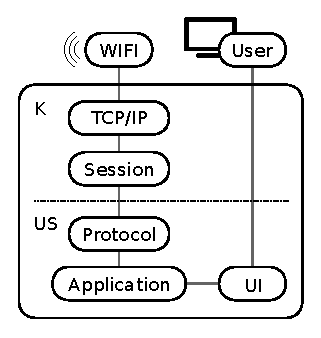
\includegraphics[width = 0.4\linewidth]{graphics/stationary_software.eps}
	\caption{Structure of software on stationary computer.}
	\label{fig:setup_ui}
\end{figure}

\subsection{Protocol}
As described in section \ref{sec:canbusanalysis}, a custom protocol will be developed to complement CAN.
Any data received through the WiFi will be encoded using this protocol.
It is the responsibility of this software to decode the software in order to present it to the user in a readable format.
In order to maintain the modularity of the system, the decoding should be done in such a way that future developers can easily add new nodes, and with them, new decoding for data types.

\subsection{Application}
The system is intended to function as a monitoring system of go-kart data.
Presentation of the data is not the focus of the project and as such only a rudimentary UI is developed to show the functionality.
The software should however be designed in such a way that a developer can easily create a custom (G)UI for the system, which fits the needs of that particular project.
In order to create the most seamless interface for this functionality the software should implement an API which acts as a front end for the underlying network.
The API-approach has the added benefit of allowing the user to use the incoming data in any way that may suit their project.


\section{Conclusion}
\label{sec:analysisconclusion}
In the analysis, a number of decisions were taken in order to give a preliminary design. \\

A number of parameters of interest were explored, eventually resulting in three types of sensors to be implemented, an IMU, a GPS and the motor controller.
These were the VN-100 from Vectornav, the NEO-6P from U-blox and the Sevcon Gen4, all of which were available from SDU.
Based on these sensors, the expected data rate was found to be 86.4 kb/s.
It was decided to make a distributed network of embedded platforms. 
CAN bus was selected to handle communication between these.\\

For implementation, the embedded platform has been selected to be the Zybo from Diligent, running Xillinux.
The wireless data connection between the go-kart and the stationary computer will be handled using WiFi.
The SD card with Linux mounted in each Zybo has sufficient free storage for logging data at a high rate.
A Linux based computer will be used to receive data wirelessly from the go-kart, and present it to a user. \\

These decisions resulted in a list of requirements, as seen in section~\ref{sec:system_requirements}.
A full overview of the system is displayed in table~\ref{fig:complete_system}.
% section system_analysis (end)